\documentclass[11pt,a4paper,]{article}
\usepackage{lmodern}

\usepackage{amssymb,amsmath}
\usepackage{ifxetex,ifluatex}
\usepackage{fixltx2e} % provides \textsubscript
\ifnum 0\ifxetex 1\fi\ifluatex 1\fi=0 % if pdftex
  \usepackage[T1]{fontenc}
  \usepackage[utf8]{inputenc}
\else % if luatex or xelatex
  \usepackage{unicode-math}
  \defaultfontfeatures{Ligatures=TeX,Scale=MatchLowercase}
\fi
% use upquote if available, for straight quotes in verbatim environments
\IfFileExists{upquote.sty}{\usepackage{upquote}}{}
% use microtype if available
\IfFileExists{microtype.sty}{%
\usepackage[]{microtype}
\UseMicrotypeSet[protrusion]{basicmath} % disable protrusion for tt fonts
}{}
\PassOptionsToPackage{hyphens}{url} % url is loaded by hyperref
\usepackage[unicode=true]{hyperref}
\hypersetup{
            pdftitle={Analysis on CO2 Emission, Population and Energy Use Problems},
            pdfborder={0 0 0},
            breaklinks=true}
\urlstyle{same}  % don't use monospace font for urls
\usepackage{geometry}
\geometry{a4paper, centering, text={16cm,24cm}}
\usepackage[style=authoryear-comp,]{biblatex}
\addbibresource{references.bib}
\usepackage{longtable,booktabs}
% Fix footnotes in tables (requires footnote package)
\IfFileExists{footnote.sty}{\usepackage{footnote}\makesavenoteenv{long table}}{}
\IfFileExists{parskip.sty}{%
\usepackage{parskip}
}{% else
\setlength{\parindent}{0pt}
\setlength{\parskip}{6pt plus 2pt minus 1pt}
}
\setlength{\emergencystretch}{3em}  % prevent overfull lines
\providecommand{\tightlist}{%
  \setlength{\itemsep}{0pt}\setlength{\parskip}{0pt}}
\setcounter{secnumdepth}{5}

% set default figure placement to htbp
\makeatletter
\def\fps@figure{htbp}
\makeatother


\title{Analysis on CO2 Emission, Population and Energy Use Problems}

%% MONASH STUFF

%% CAPTIONS
\RequirePackage{caption}
\DeclareCaptionStyle{italic}[justification=centering]
 {labelfont={bf},textfont={it},labelsep=colon}
\captionsetup[figure]{style=italic,format=hang,singlelinecheck=true}
\captionsetup[table]{style=italic,format=hang,singlelinecheck=true}


%% FONT
\RequirePackage{bera}
\RequirePackage[charter,expert,sfscaled]{mathdesign}
\RequirePackage{fontawesome}

%% HEADERS AND FOOTERS
\RequirePackage{fancyhdr}
\pagestyle{fancy}
\rfoot{\Large\sffamily\raisebox{-0.1cm}{\textbf{\thepage}}}
\makeatletter
\lhead{\textsf{\expandafter{\@title}}}
\makeatother
\rhead{}
\cfoot{}
\setlength{\headheight}{15pt}
\renewcommand{\headrulewidth}{0.4pt}
\renewcommand{\footrulewidth}{0.4pt}
\fancypagestyle{plain}{%
\fancyhf{} % clear all header and footer fields
\fancyfoot[C]{\sffamily\thepage} % except the center
\renewcommand{\headrulewidth}{0pt}
\renewcommand{\footrulewidth}{0pt}}

%% MATHS
\RequirePackage{bm,amsmath}
\allowdisplaybreaks

%% GRAPHICS
\RequirePackage{graphicx}
\setcounter{topnumber}{2}
\setcounter{bottomnumber}{2}
\setcounter{totalnumber}{4}
\renewcommand{\topfraction}{0.85}
\renewcommand{\bottomfraction}{0.85}
\renewcommand{\textfraction}{0.15}
\renewcommand{\floatpagefraction}{0.8}


%\RequirePackage[section]{placeins}

%% SECTION TITLES


%% SECTION TITLES (NEW: Changing sections and subsections color)
\RequirePackage[compact,sf,bf]{titlesec}
\titleformat*{\section}{\Large\sf\bfseries\color[rgb]{0.8, 0.7, 0.1 }}
\titleformat*{\subsection}{\large\sf\bfseries\color[rgb]{0.8, 0.7, 0.1 }}
\titleformat*{\subsubsection}{\sf\bfseries\color[rgb]{0.8, 0.7, 0.1 }}
\titlespacing{\section}{0pt}{2ex}{.5ex}
\titlespacing{\subsection}{0pt}{1.5ex}{0ex}
\titlespacing{\subsubsection}{0pt}{.5ex}{0ex}


%% TITLE PAGE
\def\Date{\number\day}
\def\Month{\ifcase\month\or
 January\or February\or March\or April\or May\or June\or
 July\or August\or September\or October\or November\or December\fi}
\def\Year{\number\year}

%% LINE AND PAGE BREAKING
\sloppy
\clubpenalty = 10000
\widowpenalty = 10000
\brokenpenalty = 10000
\RequirePackage{microtype}

%% PARAGRAPH BREAKS
\setlength{\parskip}{1.4ex}
\setlength{\parindent}{0em}

%% HYPERLINKS
\RequirePackage{xcolor} % Needed for links
\definecolor{darkblue}{rgb}{0,0,.6}
\RequirePackage{url}

\makeatletter
\@ifpackageloaded{hyperref}{}{\RequirePackage{hyperref}}
\makeatother
\hypersetup{
     citecolor=0 0 0,
     breaklinks=true,
     bookmarksopen=true,
     bookmarksnumbered=true,
     linkcolor=darkblue,
     urlcolor=blue,
     citecolor=darkblue,
     colorlinks=true}

\usepackage[showonlyrefs]{mathtools}
\usepackage[no-weekday]{eukdate}

%% BIBLIOGRAPHY

\makeatletter
\@ifpackageloaded{biblatex}{}{\usepackage[style=authoryear-comp, backend=biber, natbib=true]{biblatex}}
\makeatother
\ExecuteBibliographyOptions{bibencoding=utf8,minnames=1,maxnames=3, maxbibnames=99,dashed=false,terseinits=true,giveninits=true,uniquename=false,uniquelist=false,doi=false, isbn=false,url=true,sortcites=false}

\DeclareFieldFormat{url}{\texttt{\url{#1}}}
\DeclareFieldFormat[article]{pages}{#1}
\DeclareFieldFormat[inproceedings]{pages}{\lowercase{pp.}#1}
\DeclareFieldFormat[incollection]{pages}{\lowercase{pp.}#1}
\DeclareFieldFormat[article]{volume}{\mkbibbold{#1}}
\DeclareFieldFormat[article]{number}{\mkbibparens{#1}}
\DeclareFieldFormat[article]{title}{\MakeCapital{#1}}
\DeclareFieldFormat[article]{url}{}
%\DeclareFieldFormat[book]{url}{}
%\DeclareFieldFormat[inbook]{url}{}
%\DeclareFieldFormat[incollection]{url}{}
%\DeclareFieldFormat[inproceedings]{url}{}
\DeclareFieldFormat[inproceedings]{title}{#1}
\DeclareFieldFormat{shorthandwidth}{#1}
%\DeclareFieldFormat{extrayear}{}
% No dot before number of articles
\usepackage{xpatch}
\xpatchbibmacro{volume+number+eid}{\setunit*{\adddot}}{}{}{}
% Remove In: for an article.
\renewbibmacro{in:}{%
  \ifentrytype{article}{}{%
  \printtext{\bibstring{in}\intitlepunct}}}

\AtEveryBibitem{\clearfield{month}}
\AtEveryCitekey{\clearfield{month}}

\makeatletter
\DeclareDelimFormat[cbx@textcite]{nameyeardelim}{\addspace}
\makeatother

\author{\sf\Large\textbf{ Yu Luo}\\ {\sf\large Master\\[0.5cm]} \sf\Large\textbf{ Khushee Thakker}\\ {\sf\large Master\\[0.5cm]} \sf\Large\textbf{ Yunqi Chen}\\ {\sf\large Master\\[0.5cm]}}

\date{\sf\Date~\Month~\Year}
\makeatletter
\lfoot{\sf Luo, Thakker, Chen: \@date}
\makeatother


%%%% PAGE STYLE FOR FRONT PAGE OF REPORTS

\makeatletter
\def\organization#1{\gdef\@organization{#1}}
\def\telephone#1{\gdef\@telephone{#1}}
\def\email#1{\gdef\@email{#1}}
\makeatother
  \organization{the World Bank data base}

  \def\name{Machine Learning \hbox{Consulting \&} \hbox{ and Visualization}}    %NEW: Adding new department

  \telephone{(03) 9905 2478}

  \email{questions@company.com}                 %NEW: New email addresss

\def\webaddress{\url{http://company.com/stats/consulting/}} %NEW: URl
\def\abn{12 377 614 630}                                    % NEW: ABN
\def\logo{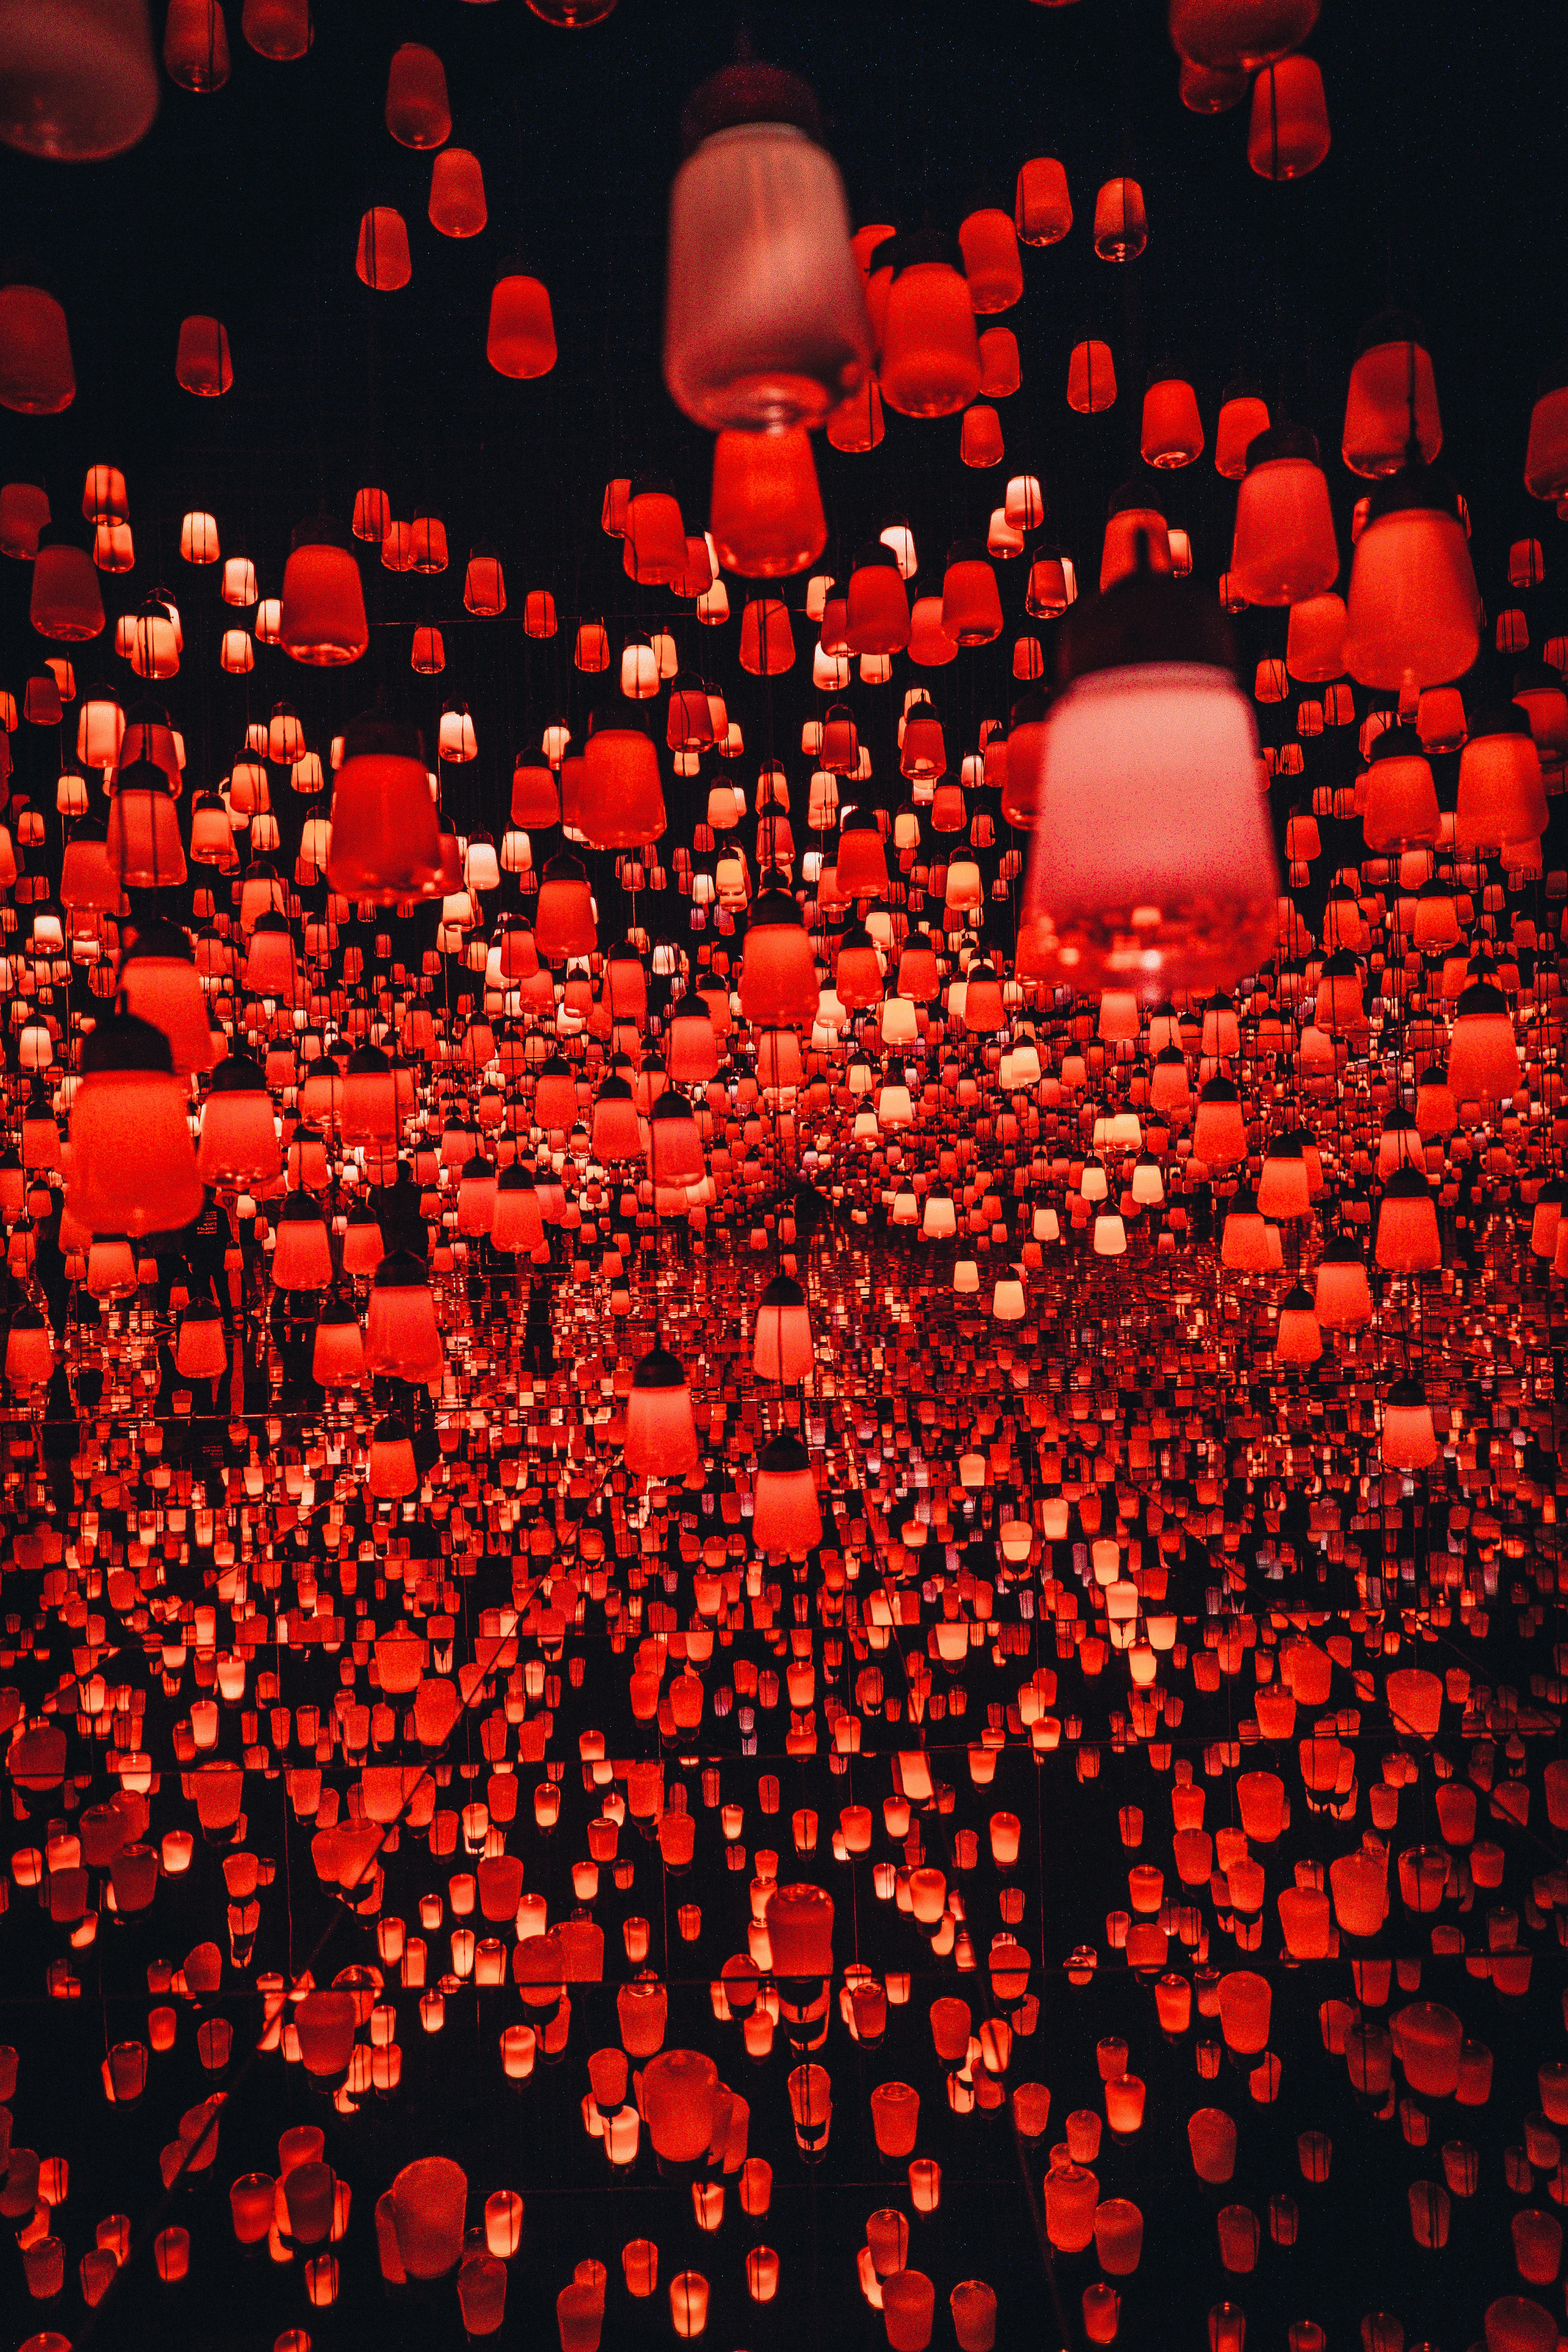
\includegraphics[width=6cm]{Figures/logo}}  %NEW: Changing logo
\def\extraspace{\vspace*{1.6cm}}
\makeatletter
\def\contactdetails{\faicon{phone} & \@telephone \\
                    \faicon{envelope} & \@email}
\makeatother

%%%% FRONT PAGE OF REPORTS

\def\reporttype{Report for}

\long\def\front#1#2#3{
\newpage
\begin{singlespacing}
\thispagestyle{empty}
\vspace*{-1.4cm}
\hspace*{-1.4cm}
\hbox to 16cm{
  \hbox to 6.5cm{\vbox to 14cm{\vbox to 25cm{
    \logo
    \vfill
    \parbox{6.3cm}{\raggedright
      \sf\color[rgb]{0.8, 0.7, 0.1 }    % NEW color 
      {\large\textbf{\name}}\par
      \vspace{.7cm}
      \tabcolsep=0.12cm\sf\small
      \begin{tabular}{@{}ll@{}}\contactdetails
      \end{tabular}
      \vspace*{0.3cm}\par
      ABN: \abn\par
    }
  }\vss}\hss}
  \hspace*{0.2cm}
  \hbox to 1cm{\vbox to 14cm{\rule{4pt}{26.8cm}\vss}\hss\hfill}  %NEW: Thicker line
  \hbox to 10cm{\vbox to 14cm{\vbox to 25cm{   
      \vspace*{3cm}\sf\raggedright
      \parbox{11cm}{\sf\raggedright\baselineskip=1.2cm
         \fontsize{24.88}{30}\color[rgb]{0, 0.29, 0.55}\sf\textbf{#1}}   % NEW: title color blue
      \par
      \vfill
      \large
      \vbox{\parskip=0.8cm #2}\par
      \vspace*{2cm}\par
      \reporttype\\[0.3cm]
      \hbox{#3}%\\[2cm]\
      \vspace*{1cm}
      {\large\sf\textbf{\Date~\Month~\Year}}
   }\vss}
  }}
\end{singlespacing}
\newpage
}

\makeatletter
\def\titlepage{\front{\expandafter{\@title}}{\@author}{\@organization}}
\makeatother

\usepackage{setspace}
\setstretch{1.5}

%% Any special functions or other packages can be loaded here.
\usepackage{booktabs}
\usepackage{longtable}
\usepackage{array}
\usepackage{multirow}
\usepackage{wrapfig}
\usepackage{float}
\usepackage{colortbl}
\usepackage{pdflscape}
\usepackage{tabu}
\usepackage{threeparttable}
\usepackage{threeparttablex}
\usepackage[normalem]{ulem}
\usepackage{makecell}
\usepackage{xcolor}


\begin{document}
\titlepage

\section*{Introduction}

This report analyzes population growth, energy use, and CO2 emissions in six countries belonging to three income groups between the 1960s-2010s. Three main sections contain the analysis of Switzerland and France from the high-income group, China and South Africa from the upper-middle-income group and Congo and Benin from the low-income group. By comparing two countries of each group, we can see the interaction effects between population growth, energy use, and CO2. It can also carry out the performance of the energy use efficiency. The source of the data is the World Bank Database.

We have used \textcite{AJMI2015629} to understand the relation between CO2 emission and energy use, and for the relationship between population and environment.

This report was written using (\textcite{R}). The following R packages were used to produce this report: \textcite{tidyverse}, \textcite{readr}, \textcite{kableExtra}, \textcite{bookdown}, \textcite{ggplot2}, \textcite{ggpubr}, \textcite{plotly}, \textcite{data}, \textcite{tidyr}, \textcite{formattable}, \textcite{stringr} and \textcite{scales}.

\section*{1 Comparison Between Two High-Income Countries: Switzerland and France}

In the high-income group countries, we pick Switzerland and France to compare their population growth, CO2 emissions and energy use. These two countries are also in the top 10 Most Green Countries in the world in Forbes rankings.

\subsection*{1.1 How is the Population and CO2 Emissions Trends in Switzerland and France?}

In order to estimate the change in population growth and CO2 emissions, we plot below figure to get a snapshot of the trends during 1960 and 2014.

\begin{figure}[!h]

{\centering \includegraphics{report_files/figure-latex/urbanco2-1} 

}

\caption{Population Growth Trends Comparison and CO2 Emissions}\label{fig:urbanco2}
\end{figure}

In Figure \ref{fig:urbanco2}, we find France has a much higher growth of population than Switzerland. From 1960s to the middle of 1970s, Switzerland had a rapid growth in CO2 emissions per capita which France had the similar one, then it went down slowly to and keep steady till 2014. Different from Switzerland, the CO2 emissions per capita of France were volatile and went back to same level of 1973 in 1979, however, after 1979, it was decreasing very fast and closes to same low level of Switzerland. This Figure shows both countries are excellent performers in CO2 emissions control since 1970s, while France did better even the population grows faster than Switzerland.

As we see in Table \ref{tab:ttlurbanco2}, during 1960s and 2000s, the total CO2 emissions billion tons per capita very decade of France is around ten times than Switzerland, and was growing due to the population growth.

\begin{table}[!h]

\caption{\label{tab:ttlurbanco2}Total CO2 Emissions Every Decade(Billion Tons per capita)}
\centering
\begin{tabular}[t]{l|r|r|r|r|r}
\hline
Country\_Name & 1960s & 1970s & 1980s & 1990s & 2000s\\
\hline
France & 2270.2236 & 3527.4263 & 3055.492 & 2733.0854 & 2870.1562\\
\hline
Switzerland & 209.9851 & 308.3635 & 295.382 & 304.4307 & 298.6183\\
\hline
\end{tabular}
\end{table}

\subsection*{1.2 How is the Energy Use and CO2 Emissions in Switzerland and France?}

Energy use is the one of the main factors that causes the CO2 Emissions. In this part, we compare the energy use and CO2 emissions per capita to present their performance in efficiency of energy use.

\begin{figure}[!h]

{\centering \includegraphics{report_files/figure-latex/energyco-1} 

}

\caption{Trends of Energy Use and CO2 Emissions Per Capita}\label{fig:energyco}
\end{figure}

Figure \ref{fig:energyco} shows France is higher than Switzerland in energy use. Since 1970, the difference between two countries in energy use per capita was going larger especially after 1090, while from 1979 on, the CO2 emissions per capita of France was decreasing and went to close Switerland. It indicates that compared with Switzerland, France use energy more efficiently after 1990.

\clearpage
\section*{2 Comparison Between Two Upper-Middle-Income Countries: China and South Africa}

\subsection*{2.1 How is the Urban Population Trend in China and South Africa?}

\begin{figure}[!h]

{\centering \includegraphics{report_files/figure-latex/fig1-1} 

}

\caption{Population Trend by Year in China and South Africa}\label{fig:fig1}
\end{figure}

As we all know, China is one of the largest population countries in the world. Moreover, China indeed has a much more considerable amount of population than South Africa. To be more specific, in Figure \ref{fig:fig1}, China has a surprising amount of population in the year 1960 with \textbf{\ensuremath{1.0808535\times 10^{8}}}. Since then, the population amount increased rapidly in the last 60 years and peaked in 2018 with \textbf{\ensuremath{8.2382765\times 10^{8}}}. On the contrary, the population amount in South Africa stayed at approximately Ten million and had a slight increase during these years. Until 2018, the population in South Africa reached \textbf{\ensuremath{3.8339668\times 10^{7}}}.

\subsection*{2.2 Does Energy Use (kg of oil equivalent per capita) Related to CO2 Emissions (metric tons per capita)?}

\begin{enumerate}
\def\labelenumi{(\arabic{enumi})}
\tightlist
\item
  A glance at the CO2 emission situation in the recent 60 years in China and South Africa.
\end{enumerate}

\begin{table}[!h]

\caption{\label{tab:tab1}CO2 Emissions Situation by Decades in China and South Africa}
\centering
\begin{tabular}[t]{l|r|r}
\hline
Decade & China & South Africa\\
\hline
1960s & 0.7214684 & 6.263097\\
\hline
1970s & 1.2257540 & 7.374369\\
\hline
1980s & 1.8054809 & 9.409576\\
\hline
1990s & 2.5445296 & 8.489207\\
\hline
2000s & 4.2558551 & 8.987882\\
\hline
2010s & 7.2655810 & 8.968759\\
\hline
\end{tabular}
\end{table}

In Table \ref{tab:tab1}, in the 1960s, CO2 emissions (metric tons per capita) of China was comparably very low with \textbf{0.7214684}, while South Africa's was around 6 times larger. Until the 2010s, CO2 emissions of China increased approximately 7 times to \textbf{7.265581}, while South Africa's is \textbf{8.9878821}.

\begin{enumerate}
\def\labelenumi{(\arabic{enumi})}
\setcounter{enumi}{1}
\tightlist
\item
  A glance at the energy use situation in the recent 50 years in China and South Africa.
\end{enumerate}

\begin{table}[!h]

\caption{\label{tab:tab2}Energy Use Situation by Decades in China and South Africa}
\centering
\begin{tabular}[t]{l|r|r}
\hline
Decade & China & South Africa\\
\hline
1970s & 532.2289 & 2114.601\\
\hline
1980s & 655.4267 & 2601.700\\
\hline
1990s & 822.8895 & 2456.338\\
\hline
2000s & 1318.9548 & 2638.689\\
\hline
2010s & 2129.3727 & 2683.906\\
\hline
\end{tabular}
\end{table}

In Table \ref{tab:tab2}, like CO2 emission, the energy use situation in China climbed year by year since the 1970s, peaked at 2010s with \textbf{2129.3726964}. In South Africa, the energy use situation fluctuated around 2500 and peaked at \textbf{2683.9063113} in the 2010s.

\begin{enumerate}
\def\labelenumi{(\arabic{enumi})}
\setcounter{enumi}{2}
\tightlist
\item
  The possible relationship between CO2 emissions and the population.
\end{enumerate}

\begin{figure}[!h]

{\centering \includegraphics{report_files/figure-latex/fig2-1} 

}

\caption{CO2 Emission and Energy Use Trend by Year}\label{fig:fig2}
\end{figure}

Figure \ref{fig:fig2} contains the line graph of urban population trend by year and CO2 emission trend by year for China with solid lines and South Africa with dashed lines. As for China, two solid lines look similar. They all generally went up from 1970 to 2003 at a low speed. Since then, it has increased rapidly. For South Africa, the CO2 emission line and energy use line successively peaked. One is around 1980 to 1990. The other is around 1980 to 1990 and 2006 to 2010.

\clearpage
\section*{3 Comparison Between Two Lower-Income Countries: Congo, Dem. Rep. and Benin}

Congo, Dem. Rep.~and Benin are countries that come under low income groups.

\subsection*{3.1 Does CO2 Emissions (metric tons per capita) related to the Popultaion trend?}

\begin{figure}[!h]

{\centering \includegraphics{report_files/figure-latex/emission-1} 

}

\caption{CO2 emissions related to the popultaion trend}\label{fig:emission}
\end{figure}

We can observe from figure \ref{fig:emission} population growth for Congo is increased drastically from 1971 to 2014 but the CO2 emissions have shown a downward trend.
Benin has comparatively very less population than Congo still emits double amount of CO2.

\begin{table}[!h]

\caption{\label{tab:co2table}Total CO2 Emissions Every Decade}
\centering
\begin{tabular}[t]{ccc}
\toprule
Decade & Benin & Congo, Dem. Rep.\\
\midrule
1970s & 0.7039211 & 7.756181\\
1980s & 1.7018481 & 10.732566\\
1990s & 4.1895203 & 7.573188\\
2000s & 12.3302054 & 4.986441\\
2010s & 12.3649822 & 6.271155\\
\bottomrule
\end{tabular}
\end{table}

Table \ref{tab:co2table} shows the total CO2 emission with respect to population every decade. In the 2000s we can observe Benin CO2 emissions have shoot up.

\subsection*{3.2 Does energy use (kg of oil equivalent per capita) related to the population trend?}

\begin{figure}[!h]

{\centering \includegraphics{report_files/figure-latex/energyplot-1} 

}

\caption{energy use related to popultaion trend}\label{fig:energyplot}
\end{figure}

The energy usage of Congo and Benin is quite similar. Benin's energy usage is a little more than Congo.
If take population into consideration the energy usage of Benin way more in comparison of its population.
Figure \ref{fig:energyplot} represents the Energy usage is not dependent on the population growth for Benin and Congo.

\begin{table}[!h]

\caption{\label{tab:energytable}Energy Usage of Oil Every Decade}
\centering
\begin{tabular}[t]{ccc}
\toprule
Decade & Benin & Congo, Dem. Rep.\\
\midrule
1970s & 371.9804 & 324.8007\\
1980s & 352.9283 & 331.8185\\
1990s & 332.7716 & 315.2343\\
2000s & 334.7856 & 302.3236\\
2010s & 403.3246 & 355.3209\\
\bottomrule
\end{tabular}
\end{table}

Table \ref{tab:energytable} illustrates mean of energy usage per decade for Benin and Congo.

\subsection*{3.3 Trends of Energy Use and CO2 Emissions Per Capita}

\begin{figure}[!h]

{\centering \includegraphics{report_files/figure-latex/energyemission-1} 

}

\caption{Trends of Energy Use and CO2 Emissions Per Capita}\label{fig:energyemission}
\end{figure}

From Figure \ref{fig:energyemission} we observe CO2 emision show a upward trend for Benin even though there was a drop of energy usage in 2000s.
Whereas Congo shows a downward trend for CO2 emission even if there was a sudden spike in the use of energy after 2010.

\printbibliography

\end{document}
